\chapter{La Macchina di Turing} \label{ch:capitolo3}
\begin{figure}[htp]
    \centering
     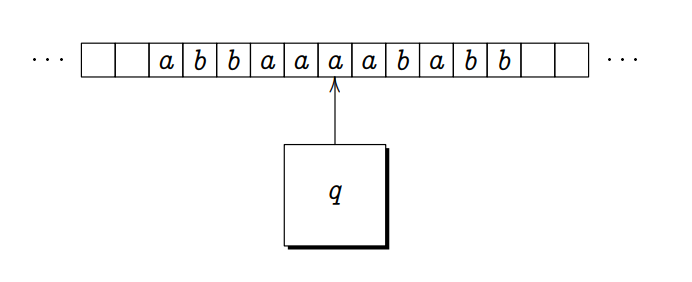
\includegraphics[scale=0.7]{tesi_stile/img/turing.png}
\end{figure}
E' composta da: 
\begin{itemize}
    \item un unità di controllo a stati finiti che
    \begin{itemize}
    
        \item può spostare il nastro a destra o a sinistra (una cella alla volta)
        
        \item contiene il programma secondo cui verrà eseguito il calcolo
        
        \item registra lo stato della macchina
        
        \item L’insieme di possibili stati della macchina è un insieme finito\\Q = \{q0, q1 ,. . . qn\}
    \end{itemize}
    \newpage
    \item un nastro di lunghezza infinita che
    
    \begin{itemize}
        \item è suddiviso in celle
        
        \item ogni cella può contenere un solo simbolo di un fissato alfabeto A, oppure essere bianca.
        
        \item  solo un numero finito di celle contiene una lettera di A.
    \end{itemize}
    
    \item Testina di lettura e scrittura
    
    \begin{itemize}
        \item che permette all’unità di controllo di leggere e scrivere un simbolo per volta dal nastro
    \end{itemize}
    
\end{itemize}
\subsection{Funzionamento}
All'avvio di ogni computazione, la macchina si trova in uno stato iniziale prefissato.\\ A ogni passo l’unità di controllo in funzione dello stato in cui si trova e del simbolo contenuto nella cella che la testina indica:
\begin{itemize}
    \item Rivede il suo stato.
    
    \item Scrive un simbolo nella cella indicata dalla testina, sostituendo il simbolo esistente (eventualmente bianco);
    
    \item Sposta la testina di una posizione a sinistra o a destra.
\end{itemize}
Il nuovo stato assunto dall'unità di controllo, il simbolo da scrivere sulla cella indicata dalla testina e lo spostamento della testina a sinistra o a destra sono determinati dal programma della macchina.
\newpage
\subsection{Programma}
Il programma di una macchina di Turing si può rappresentare come una lista di 5-ple (istruzioni):\\
$$(q,a,q',a',x)$$
\begin{itemize}
    \item q è lo stato dell'unità di controllo
    \item a l simbolo nella cella indicata dalla testina
    \item $q'$ l nuovo stato che la macchina deve assumere
    \item $a'$ la lettera da scrivere nella cella esaminata
    \item x è la testina. 
    
    Se $x = -1$ spostamento della testina a sx, $x = +1$ spostamento della testina a dx
\end{itemize} 
Per ogni coppia (q, a) ci deve essere al più una 5-pla (q, a, $q'$, $a'$, x ) nel programma della macchina \textbf{(determinismo)}
\subsection{Definizione Formale}
\textbf{Definizione}\\
Una macchina di Turing M è una quadrupla:
\begin{center}
    $$M=<Q,A,\delta,q_0>$$
\end{center}
\begin{itemize}
    \item $Q$ è un insieme finito di stati
    \item $A$ è un alfabeto a cui si aggiunge il simbolo \textit{bianco} \#
    \item $\delta$ è una funzione \textbf{parziale} da $Q \times (A \cup \{\# \})$ a \\
    $Q \times (A \cup \{\# \}) \times \{-1,+1\}$
    \item $q_0 \in Q$ è lo stato iniziale
\end{itemize}
Le 5-ple (q, a, $q'$, $a'$, x ) tali che $\delta$(q,a) = ($q'$, $a'$, x) sono dette \textbf{istruzioni} di M.
\subsection{Configurazione istantanea}
Lo stato di una Macchina di Turing a un dato istante può essere descritta da una 4-pla:
\begin{center}
   $$C_i = (\xi,q,a,\eta)$$ 
\end{center}
\begin{itemize}
    \item $\xi \ (xi)$ è il contenuto del nastro a sinistra della cella indicata dalla testina, privato della sequenza infinita di celle bianche che precedono l’ultimo simbolo non bianco. \emoji{orangutan}: $\xi$ contiene tutte le lettere a sinistra della testina fino alle infinite celle bianche (il nastro \`{e} infinito sia a destra che a sinistra)
    
    \item q è lo stato della Macchina di Turing nell’istante considerato
    
    \item a è la lettera nella cella indicata dalla testina
    
    \item $\eta \ (eta)$ è il contenuto del nastro a destra della cella indicata dalla testina, privato della sequenza infinita di celle bianche che seguono l’ultimo simbolo non bianco. \emoji{orangutan}: \`{e} come $\xi$ ma a destra
\end{itemize}
\textbf{Esempio}
\vspace{0.2cm}
\begin{figure}[htp]
    \centering
     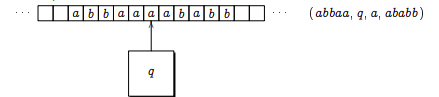
\includegraphics[scale=0.7]{tesi_stile/img/ese-turing.png}
\end{figure}
\newpage
\subsection{Configurazione consecutiva}
Una configurazione istantanea di una Macchina di Turing $$M=<Q,A,\delta,q_0>$$ è un elemento dell’insieme (A U \{\#\})* × Q × (A U \{\#\}) × (A U \{\#\})*.\\
Nell’insieme delle configurazioni istantanee di M introduciamo la relazione binaria  $\vdash_M$  che associa alla configurazione C quella che la segue nella computazione di M. Qualora tale configurazione non esistesse, scriveremo $\vdash/_M$.\\\\
\textbf{Esempio}\\
Se M ha l’istruzione (q, a, $q$, b, $-$1), allora:
\begin{center}
    (abbaa, q, a, ababb) $\vdash_M$ (abba, $q'$, a, bababb)
\end{center}
\subsection{Computazione}
\begin{itemize}
    \item Al passo iniziale 
    
    \begin{itemize}
    \item M esamina una parola w scritta sul nastro di input.
    
    \item La testina indica la prima lettera di w.
    
    \item Lo stato è lo stato iniziale q0.
    
    \item la configurazione istantanea iniziale è ($\wedge$, q0, a, $w'$), ove w = a$w'$ con a lettera
    \end{itemize}
\end{itemize}
\begin{itemize}
    \item Se all’istante i, M si trova nella configurazione C$_i$ e C$_i$  $\vdash_M$ C$_i$+1, allora all’istante i+1 M sarà nella configurazione C$_i$+1.
    
    \item Se invece C$_i$ $\vdash/_M$, allora la macchina si arresta.
    
    \item Se M si arresta dopo un numero finito di passi diremo che M converge sull’input w e scriveremo M $\downarrow$ w, in caso contrario diremo che M diverge sull’input w e scriveremo M $\uparrow$ w.
\end{itemize}
\newpage
\textbf{Esempio: bitwise not}
\begin{figure}[htp]
    \centering
     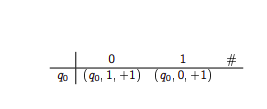
\includegraphics[scale=0.9]{tesi_stile/img/bit.png}
\end{figure}

\textbf{Esempio: palindrome}
\begin{figure}[htp]
    \centering
     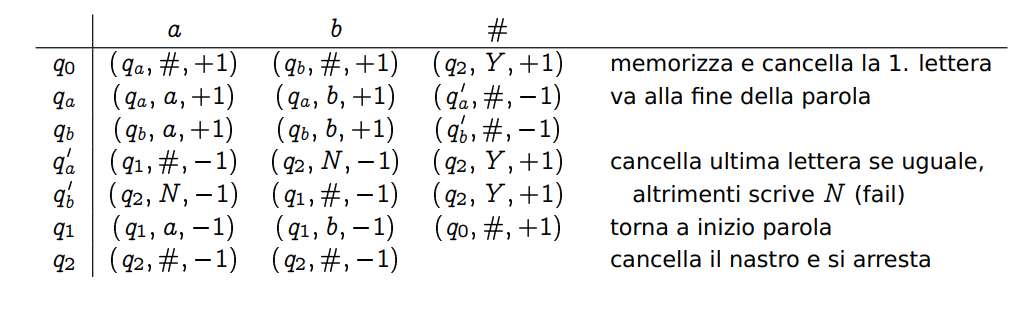
\includegraphics[scale=0.6]{tesi_stile/img/pal.png}
\end{figure}
\newpage
\subsection{Algoritmi e macchina di Turing}
\begin{figure}[htp]
    \centering
     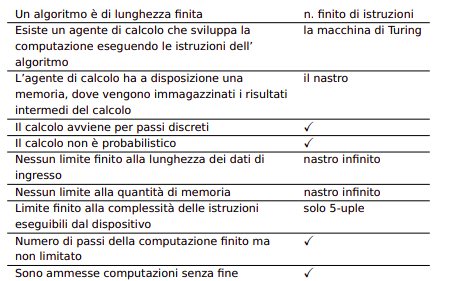
\includegraphics[scale=1]{tesi_stile/img/algo-turing.png}
\end{figure}
\subsection{L'impiegato diligente}
La macchina di turing è un Meccanismo che simuli le potenzialità computazionali dell’uomo comune quindi: 
\begin{itemize}
    \item Esegue ordinatamente le sue istruzioni, purché non siano tra loro in concorrenza.
    
    \item In assenza di istruzioni si arresta.
\end{itemize}
\newpage
\subsection{Macchina di turing e linguaggi}
Come detto in precendeza:
\begin{itemize}
    \item La configurazione istantanea iniziale è C0 = ($\wedge$, q0, a, $w'$), ove w = a$w'$
    con a lettera.
    
    \item Se C$_0$ $\vdash_M$ C$_1$ $\vdash_M$ ... $\vdash_M$ $C_n$ $\vdash/_M$ M allora M \textbf{converge} sull’input w.
    
    \item Se C$_0$ $\vdash_M$ C$_1$ $\vdash_M$ ... $\vdash_M$ $C_n$ $\vdash_M$ M allora M \textbf{diverge} sull’input w.
\end{itemize}
\textbf{Definizioni}\\
Sia L un linguaggio sull’alfabeto A.
\begin{enumerate}
    \item Una macchina di Turing M accetta il linguaggio L se M \textbf{converge su tutti gli input} w $\in$ L e \textbf{diverge} su tutti gli input w $\not \in$ L.
    
    \item Una macchina di Turing M decide il linguaggio L se M \textbf{converge su tutti gli input} w $\in$ A* con output SI se w $\in$ L e NO se w $\not \in$ L.
\end{enumerate}
\subsection{Problemi decidibili}
Le nozioni di linguaggio accettato e deciso sono profondamente diverse.
\begin{itemize}
    \item Entrambe definiscono correttamente un linguaggio.
    
    \item Solo la nozione di linguaggio deciso ci fornisce una procedura effettiva che, in un numero finito di passi, ci permette di dire se una parola appartiene o meno al linguaggio.
\end{itemize}
\textbf{Definizione}\\
Un linguaggio L si dice decidibile secondo Turing se esiste una macchina di Turing M che decide L, indecidibile (secondo Turing) altrimenti.\\
Un linguaggio L si dice semidecidibile secondo Turing se esiste una macchina di Turing M che accetta L.\\\\
\textbf{Proposizione}\\
Un linguaggio decidibile è anche semidecidibile\\\\
\textbf{Dimostrazione}\\
Trasformare la macchina che decide L in una che accetta L, aggiungendo un loop infinito se la macchina originale si arresta sul NO.\\\\
\textbf{Esempio}
\begin{figure}[htp]
    \centering
     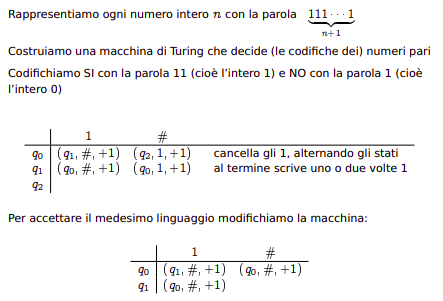
\includegraphics[scale=0.9]{tesi_stile/img/esempio.png}
\end{figure}
\subsection{Aritmetizzazione della macchina di turing}
\textbf{Obbietivo}\\
\begin{itemize}
    \item Associare un numero a ogni input e output di una macchina di Turing.
    
    \item Associare un numero (indice) a ogni macchina di Turing.
    
    \item In maniera effettiva:
    
    \begin{itemize}
        \item Data una macchina di Turing, ne posso calcolare l’indice.
        
        \item Dato un indice, posso calcolare le istruzioni della macchina corrispondente.
    \end{itemize}
\end{itemize}
\textbf{Una prima strategia}
\begin{itemize}
    \item Ordinare le parole nell’ordine militare.
    
    \item Associare a ogni parola la sua posizione nell’elenco ordinato.
\end{itemize}

Oppure

\begin{itemize}
    \item Interpretare ogni lettera come una cifra $\neq$ 0 di un sistema numerico.
    
    \item Associare a ogni parola il numero corrispondente.
\end{itemize}

\subsection{Numerazione di i Gödel}
Metodo per numerare gli alberi (con foglie etichettate).
\begin{figure}[htp]
    \centering
     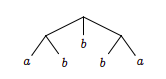
\includegraphics[scale=1]{tesi_stile/img/goedel.png}
\end{figure}
\begin{itemize}
    \item A ogni etichetta x associo un numero dispari G$_0$(x) $>=$ 3
    
    \item A un albero T di altezza 1, con foglie etichettate x$_1$, x$_2$, ... , x$_k$ associo il numero $$G_1(T) = 2^{G_0(x_1)} \cdot 3^{G_0(x_2)} \cdot 5^{G_0(x_3)} \cdot ... \cdot P_n^{G_0(x_k)}$$ dove 2, 3, ..., p$_k$ è la sequenza dei primi k numeri primi
    
    \item In generale, se la radice dell’albero T ha, da sinistra a destra, i figli v$_1$, . . . , v$_t$, radici di sottoalberi alberi con numeri di Gödel n$_1$, . . . , n$_t$, allora il numero di Gödel di T è 2$^{n1}$ 3$^{n2}$...p$_t^{ni}$
\end{itemize}
\newpage
\textbf{Esempio}\\
Posso anche fare il percorso inverso:
\begin{itemize}
    \item Un numero dispari rappresenta una foglia.
    
    \item Un numero pari va decomposto come prodotto di potenze di primi.
    
    \item Gli esponenti sono i numeri di Gödel dei sottoalberi
\end{itemize}
Posso quindi distinguere gli interi che non sono numeri di Gödel.\\\\
\begin{figure}[htp]
    \centering
     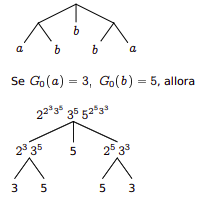
\includegraphics[scale=1]{tesi_stile/img/inverso.png}
\end{figure}\\
\textbf{Il Teorema Fondamentale dell’Aritmetica assicura che la decodifica è unica.}
\newpage
\subsection{Numerazione della macchina di turing}
Una macchina di Turing è rappresentata da una lista di 5-ple e, in definitiva, da un albero.\\\\
\textbf{Esempio}\\
La macchina che accetta i numeri pari ha le 5-ple (in ordine lessicografico).\\
\begin{center}
    (q$_0$, \#, q$_0$, \#, $+1$),(q$_0$, 1, q$_1$, \#, $+1$),(q$_1$, 1, q$_0$, \#, $+1$)
\end{center}
Possiamo identificarlo come albero:
\begin{figure}[htp]
    \centering
     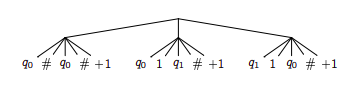
\includegraphics[scale=1]{tesi_stile/img/albero.png}
\end{figure}\\
Per numerare le macchine di Turing su un alfabeto A,\\ 
associamo: un intero dispari $>$ 1 a ognuno dei simboli necessari.\\
\begin{figure}[htp]
    \centering
     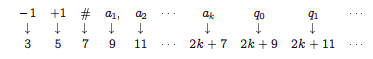
\includegraphics[scale=0.8]{tesi_stile/img/numeri.png}
\end{figure}
\newpage
Per ogni macchina di Turing M:
\begin{itemize}
    \item Ordiniamo le 5-ple in ordine lessicografico.
    
    \item Calcoliamo il numero di Gödel dell’albero corrispondente.\\
    \begin{figure}[htp]
        \centering
        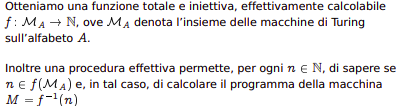
\includegraphics[scale=0.9]{tesi_stile/img/sotto.png}
     
    \end{figure}
\end{itemize}
\begin{figure}[htp]
    \centering
    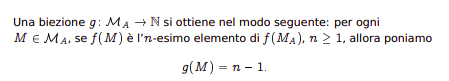
\includegraphics[scale=0.9]{tesi_stile/img/biiezione.png}
\end{figure}
\textbf{Osservazione}\\
Una procedura effettiva per calcolare x = g(M) è la seguente:
\begin{figure}[htp]
    \centering
    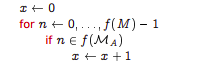
\includegraphics[scale=0.8]{tesi_stile/img/algoritmo.png}
\end{figure}\\
\textbf{Teorema}\\
C’è una corrispondenza biunivoca effettiva tra le macchine di Turing su un alfabeto A e i numeri naturali.
\newpage
\subsection{Coppie di interi}
\textbf{Teorema di Cantor:} Esiste una biiezione effettiva tra $N^2$ ed $N$ data da:\\
$$(n,m)=\frac{(n+m)(n+m+1)}{2}+n$$
Basta osservare che ogni naturale compare infinite volte come ascissa di una coppia $(n,m) \in N^2$ al variare di $m$, intuitivamente quindi ci sono tante coppie ordinate di naturali quanti naturali.
\begin{figure}[htp]
    \centering
    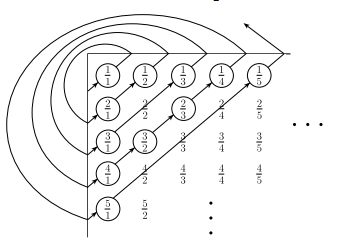
\includegraphics[scale=0.9]{tesi_stile/img/cantor.png}
\end{figure}\\
\textbf{Corollario}\\
C’è una corrispondenza biunivoca effettiva tra le macchine di Turing su qualsiasi alfabeto e i numeri naturali.
Per il teorema precedente possiamo enumerare le macchine di Turing
\begin{center}
    M$_0$,M$_1$,...,    M$_n$
\end{center}
Pertanto, è possibile enumerare tutte le funzioni calcolabili
\begin{center}
    $\phi_0$,$\phi_1$,...,$\phi_n$
\end{center}
Nel secondo caso, però, la corrispondenza non è biunivoca, perchè la medesima funzione può essere calcolata da più macchine di Turing.
\subsection{Descrizione delle macchine di turing}
\textbf{Descrizione formale}\\
Lista delle quintuple\\\\
\textbf{Descrizione implementativa}\\
Descrive in linguaggio corrente, il modo in cui la macchina di Turing muove la testina e registra i dati sul nastro\\\\
\textbf{Descrizione di alto livello}\\
Descrive un algoritmo, ignorando i dettagli implementativi.\\\\
\textbf{Esempio}: Palindrome\\\\
Descrizione implementativa su input w
\begin{enumerate}
    \item cancella la prima lettera
    
    \item se non ci sono altre lettere accetta
    
    \item sposta la testina alla fine della parola
    
    \item se l’ultima lettera è diversa dalla prima rifiuta
    
    \item cancella l’ultima lettera
    
    \item se non ci sono altre lettere accetta
    
    \item sposta la testina all’inizio della parola
    
    \item ricomincia dal passo 1
\end{enumerate}
Descrizione di alto livello su input w
\begin{enumerate}
    \item se l(w) $<=$ 1, accetta
    
    \item se la prima e l’ultima lettera di w sono distinte, rifiuta
    
    \item cancella la prima e l’ultima lettera di w
    
    \item ricomincia al passo 1
\end{enumerate}
\subsection{Tesi di Church-Turing}
Una funzione è calcolabile se e solo se esiste una macchina di Turing che la calcola.
\begin{figure}[htp]
    \centering
    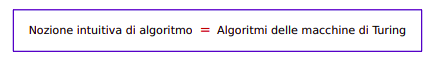
\includegraphics[scale=0.8]{tesi_stile/img/tesi.png}
\end{figure}
\textbf{Argomenti}
\begin{itemize}
    \item L’inclusione $\supseteq$ è evidente
    
    \item Assenza di controesempi
    
    \item Tecniche molto generali
    
    \item Numerosi modelli equivalenti
    
    \item Numerose generalizzazioni rivelatesi equivalenti
    
    \item La metafora dell’impiegato diligente
\end{itemize}
\textbf{Convenzione}\\
D’ora in poi considereremo solo insiemi di numeri naturali e funzioni di $N$ in $N$ (ipotesi non restrittiva). Le macchine di Turing si enumerano
\begin{center}
    M$_0$,M$_1$,...,M$_n$
\end{center}
e le funzioni da esse calcolate saranno denotate, rispettivamente
\begin{center}
    $\phi_0$,$\phi_1$,...,$\phi_n$
\end{center}
\textbf{Osservazioni}
\begin{itemize}
    \item Ogni macchina di Turing calcola una funzione (parziale) di $N$ in $N$
    
    \item Ogni macchina di Turing calcola una funzione (parziale) di $N^2$ in N
    
    \item Esiste una procedura effettiva che, data una macchina di Turing M, calcola l’indice x tale che M = M$_x$
    
    \item Esiste una procedura effettiva che, dato un numero naturale x , calcola il programma della macchina di Turing M$_x$
\end{itemize}
\subsection{Funzioni e problemi}
La funzione caratteristica di un insieme L $\subseteq$ $N$ è la funzione f$_L$ definita da:
\begin{figure}[htp]
    \centering
    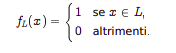
\includegraphics[scale=0.9]{tesi_stile/img/funzione.png}
\end{figure}
\textbf{Lemma}\\
Un insieme L $\subseteq$ $N$ è decidibile se e solo se la sua funzione caratteristica è computabile.\\\\
\textbf{Corollario:} Esistono insiemi indecidibili\\\\
\textbf{Dimostrazione}\\
Per il Teorema di Cantor, non ci sono ‘abbastanza’ macchine di Turing.\\\\
\textbf{Esempio}
\begin{figure}[htp]
    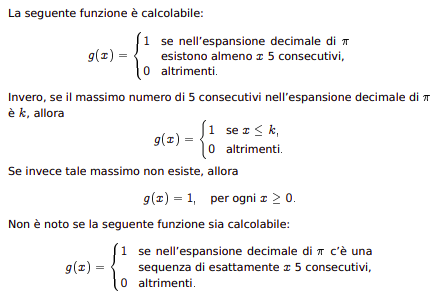
\includegraphics[scale=1]{tesi_stile/img/es-cantor.png}
\end{figure}